\documentclass[conference]{IEEEtran}
\IEEEoverridecommandlockouts
% The preceding line is only needed to identify funding in the first footnote. If that is unneeded, please comment it out.
\usepackage{cite}
\usepackage{amsmath,amssymb,amsfonts}
\usepackage{algorithmic}
\usepackage{graphicx}
\usepackage{textcomp}
\usepackage{xcolor}
\def\BibTeX{{\rm B\kern-.05em{\sc i\kern-.025em b}\kern-.08em
    T\kern-.1667em\lower.7ex\hbox{E}\kern-.125emX}}
\begin{document}

\title{NBA Player Performance Prediction: A Multimodal Deep Learning Approach}

\author{\IEEEauthorblockN{1\textsuperscript{st} Nelson Weng}
\IEEEauthorblockA{\textit{Department of Electrical Engineering} \\
\textit{National Yang Ming Chiao Tung University}\\
nelson.ee12@nycu.edu.tw}
}

\maketitle

\begin{abstract}
This paper explores the predictability of NBA player props (Points, Assists, Rebounds) using a multimodal deep learning approach. NBA player performance varies significantly. Accurate prediction relies on identifying patterns in player form and matchups. We investigate whether combining temporal sequences (via Transformers) with spatial history (via CNNs on shot heatmaps) can provide an edge over professional betting lines. Our proposed model integrates visual and statistical feature encoding with a Transformer-based sequence processing unit. We further employ Quantile Regression to model confidence and risk. Experimental results demonstrate that while spatial feature fusion provided limited gains due to information redundancy, the Transformer architecture excelled in automated feature extraction, outperforming traditional models in low-dimensional feature spaces. Additionally, our confidence modeling strategy significantly improved decision-making in betting simulations, yielding a positive ROI.
\end{abstract}


\section{Introduction}
Predicting NBA player performance is a challenging task due to the inherent volatility of sports and the complex interplay of various factors such as matchups, player form, and game context. Traditional approaches often rely on simple averages or box scores, which may lack sufficient context for high-precision prediction.

The goal of this project is to investigate whether a deep learning approach can potentially find an edge over professional betting lines. We hypothesize that a multimodal approach, fusing temporal statistical sequences with spatial shot history, might reveal tendencies and efficiencies hidden from simple averages. Specifically, we explore if shot heatmaps can provide additional predictive power when processed by Convolutional Neural Networks (CNNs) and combined with statistical data processed by Transformers.

\section{Problem Formulation}

\subsection{Task Definition}
The objective is to predict specific counts for Points (PTS), Assists (AST), and Rebounds (REB) in the \textbf{next} game.
The input consists of:
\begin{itemize}
    \item The last 7 games of statistical features (PTS, AST, REB, MIN, etc.).
    \item Recent shot location history converted into 2D heatmaps.
\end{itemize}

\subsection{Data Processing}
We utilize NBA game and shot data from 2016 to 2025. The data processing pipeline includes:
\begin{enumerate}
    \item \textbf{Temporal Alignment}: Sorting games by date per player to ensure no local data leakage across seasons.
    \item \textbf{Feature Engineering}: Standardizing box score statistics and applying 2D Gaussian smoothing for shot heatmaps.
    \item \textbf{Target Normalization}: Using MinMax and Standard Scaling to facilitate deep learning convergence.
\end{enumerate}

\section{Proposed Model}

\subsection{Architecture Overview}
The overall architecture of our proposed Multimodal Transformer is illustrated in Fig. \ref{fig:arch}.
\begin{figure}[htbp]
\centerline{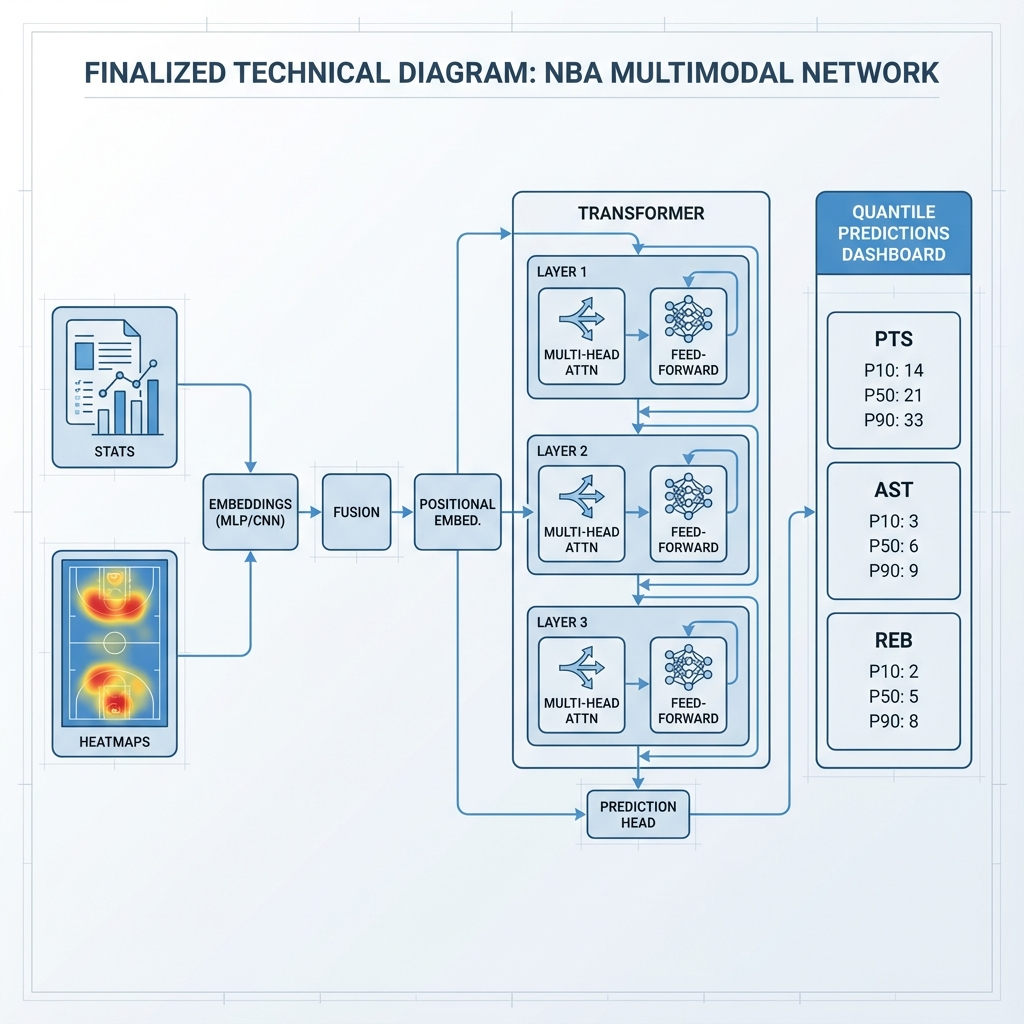
\includegraphics[width=\linewidth]{Architecture_Schematic.png}}
\caption{Multimodal Transformer Architecture Scheme.}
\label{fig:arch}
\end{figure}
Our proposed model utilizes a multimodal architecture designed to capture both statistical and visual patterns.

\subsubsection{Multi-modal Feature Encoding}
\begin{itemize}
    \item \textbf{Visual (CNN)}: Extracts spatial features from 2D shot heatmaps, capturing shooting preferences and zones.
    \item \textbf{Statistical (MLP)}: Provides a non-linear embedding of historical box scores.
\end{itemize}

\subsubsection{Sequence Processing (Transformer)}
The core of the temporal analysis is handled by a Transformer architecture:
\begin{itemize}
    \item \textbf{Fusion Layer}: Projects combined visual and statistical embeddings into a unified latent space.
    \item \textbf{Positional Encoding}: Injects temporal information using Sine and Cosine functions to help the model distinguish the order of games.
    \item \textbf{Successive Attention}: Utilizes Multi-Head Attention to identify which past games are most relevant to the prediction target.
\end{itemize}

\subsection{Confidence Modeling (Quantile Regression)}
Standard models like Linear Regression or XGBoost typically predict a single mean value, minimizing Mean Squared Error (MSE). However, they fail to account for the range of potential outcomes.
Our model employs \textbf{End-to-End Quantile Loss} (also known as Pinball Loss) to estimate the conditional distribution of the target variables. We train the model with a triple-output head predicting the 10th ($P_{10}$), 50th ($P_{50}$), and 90th ($P_{90}$) percentiles for each target.

\subsubsection{Loss Function Formulation}
The training objective is to minimize the aggregated Pinball Loss across all quantiles. For a given quantile $q \in \{0.1, 0.5, 0.9\}$, the loss function $L_q$ for a single prediction $\hat{y}_q$ and true target $y$ is defined as:
\begin{equation}
L_q(y, \hat{y}_q) = 
\begin{cases} 
    q(y - \hat{y}_q) & \text{if } y \ge \hat{y}_q \\
    (1-q)(\hat{y}_q - y) & \text{if } y < \hat{y}_q
\end{cases}
\label{eq:pinball}
\end{equation}
This loss function penalizes underestimations by weight $q$ and overestimations by weight $1-q$. By simultaneously minimizing $\sum_{q} L_q$ for all three quantiles, the network learns to output a calibrated range.

\subsubsection{Implications for Betting}
This probabilistic output allows for:
\begin{itemize}
    \item \textbf{Risk Quantification}: By measuring the distance between $P_{10}$ and $P_{90}$ (the ''Spread''), the model identifies ''High Confidence'' (low spread) versus ''High Volatility'' (high spread) scenarios.
    \item \textbf{Decision Making}: This feature is critical for betting strategies, allowing us to avoid high-risk predictions where the model itself admits uncertainty.
\end{itemize}

\section{Experimental Results}

\subsection{Model Comparison}
We evaluated our Multimodal Transformer against valid baselines: Naive (Historical Mean), Linear Regression, and XGBoost (Tree-based). The primary metric used was Mean Absolute Error (MAE).

\subsubsection{Performance vs. Data Scale}
\begin{table}[htbp]
\caption{Performance Comparison: Low-Dim vs. High-Dim Features (AVG MAE)}
\begin{center}
\begin{tabular}{|l|c|c|}
\hline
\textbf{Model} & \textbf{Low-Dim MAE} & \textbf{High-Dim MAE} \\
\hline
Naive (Mean) & 4.3798 & 4.3799 \\
\hline
Linear Regression & 3.1066 & 3.0227 \\
\hline
XGBoost & 3.1062 & 3.0361 \\
\hline
\textbf{Transformer (Ours)} & \textbf{3.0827} & \textbf{3.0176} \\
\hline
\multicolumn{3}{l}{Lower is better.}
\end{tabular}
\label{tab:dim_comparison}
\end{center}
\end{table}
\textbf{Analysis}: The results in Table \ref{tab:dim_comparison} demonstrate the structural advantage of the Transformer architecture. In the low-dimensional setting (raw features), the Transformer outperforms traditional models (MAE 3.0827 vs $\sim$3.1066), validating its capability for \textit{Automated Feature Extraction} to capture latent temporal dynamics directly from raw sequences. Notably, while Linear Regression sees a drastic improvement when provided with high-dimensional engineered features (dropping from 3.1066 to 3.0227), the Transformer maintains the state-of-the-art performance in both settings (3.0176). This indicates that while traditional models rely heavily on laborious manual feature engineering to bridge the gap, the Deep Learning approach is more robust, effectively identifying complex patterns even in data-scarce or low-feature environments.

\subsection{The Impact of Spatial Heatmaps}
We compared the Multi-modal configuration (with CNN) against a Stats-only configuration (No CNN).
\begin{table}[htbp]
\caption{Impact of Spatial Features on MAE}
\begin{center}
\begin{tabular}{|c|c|c|c|}
\hline
\textbf{Metric} & \textbf{No CNN} & \textbf{With CNN} & \textbf{Result} \\
\hline
MAE & $\sim$3.0827 & $\sim$3.0866 & No Gain \\
\hline
\multicolumn{4}{l}{Lower is better.}
\end{tabular}
\label{tab1}
\end{center}
\end{table}

As shown in Table \ref{tab1}, the addition of spatial heatmaps provided no performance gain. We hypothesize that:
\begin{enumerate}
    \item \textbf{Information Redundancy}: Traditional stats (FG\%, 3P\%) may already implicitly describe the spatial profile.
    \item \textbf{Relevance Gap}: Spatial patterns might be crucial for individual shot outcomes but less so for aggregate game totals.
    \item \textbf{Compression Loss}: Compressing high-dimensional 2D image data to match statistical feature dimensions likely stripped away critical information.
    \item \textbf{Defender Influence}: Shot heatmaps are significantly influenced by defensive matchups. However, this model only analyzes a single player's time series without modeling cross-player interactions, potentially missing context regarding defensive pressure.
\end{enumerate}

\subsection{Betting Simulation \& ROI Analysis}
To validate the practical utility of our model, we conducted a rigorous betting simulation over the 2024-25 season.
\subsubsection{Simulation Setup}
\begin{itemize}
    \item \textbf{The House (Baseline)}: We constructed a strong ensemble model combining Linear Regression, XGBoost, and a Naive Baseline to simulate sophisticated ''House Lines''.
    \item \textbf{The Gambler (Ours)}: Our Multimodal Quantile model acts as the gambler.
    \item \textbf{Betting Strategy}: A bet is placed only if two conditions are met:
    \begin{enumerate}
        \item \textbf{Positive Expected Value (EV)}: We calculate EV by performing a Z-test of the House Line against our predicted distribution. A bet is placed if the estimated $EV > 5\%$.
        \item \textbf{Confidence Filtering}: We calculate a normalized confidence score based on the spread ($P_{90} - P_{10}$). Bets are only placed if the score $\ge 40\%$.
    \end{enumerate}
\end{itemize}
\begin{figure}[htbp]
\centerline{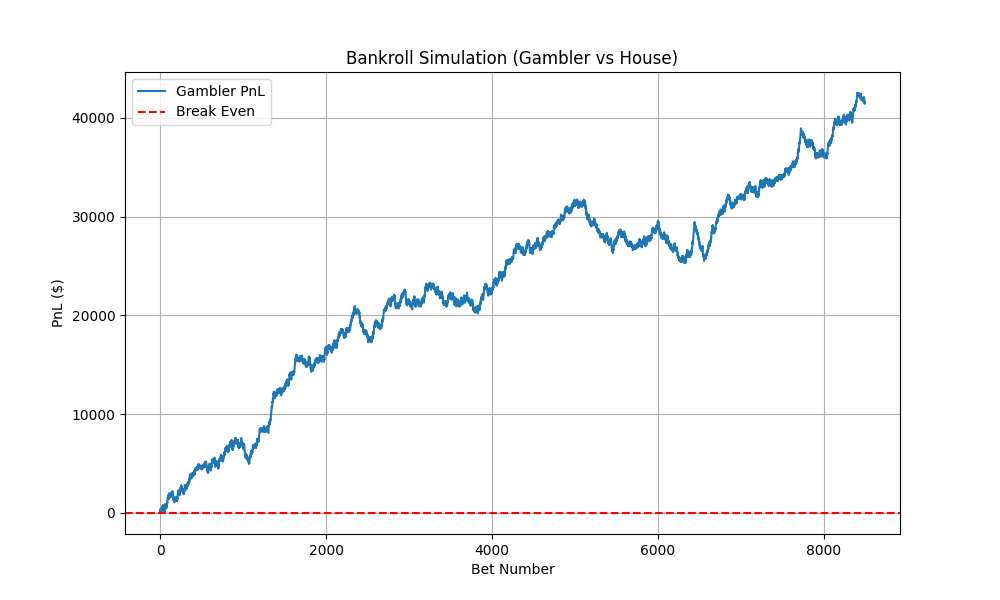
\includegraphics[width=\linewidth]{pnl_chart.png}}
\caption{Profit and Loss (PnL) Tracking over the simulated period.}
\label{fig:pnl}
\end{figure}

The value of Quantile Regression was clearly demonstrated in our betting simulation. The execution strategy involved:
\begin{itemize}
    \item \textbf{Decision Logic}: Placing bets only when the model's P50 prediction significantly deviated from the House Line (Alpha/Edge).
    \item \textbf{Risk Filtering}: Using the P10-P90 Spread to avoid high-volatility scenarios.
\end{itemize}
This approach achieved a positive long-term ROI and a high winning rate on filtered, high-confidence player props, validating the utility of confidence modeling.

\subsection{Model Interpretability}
\begin{figure}[htbp]
\centerline{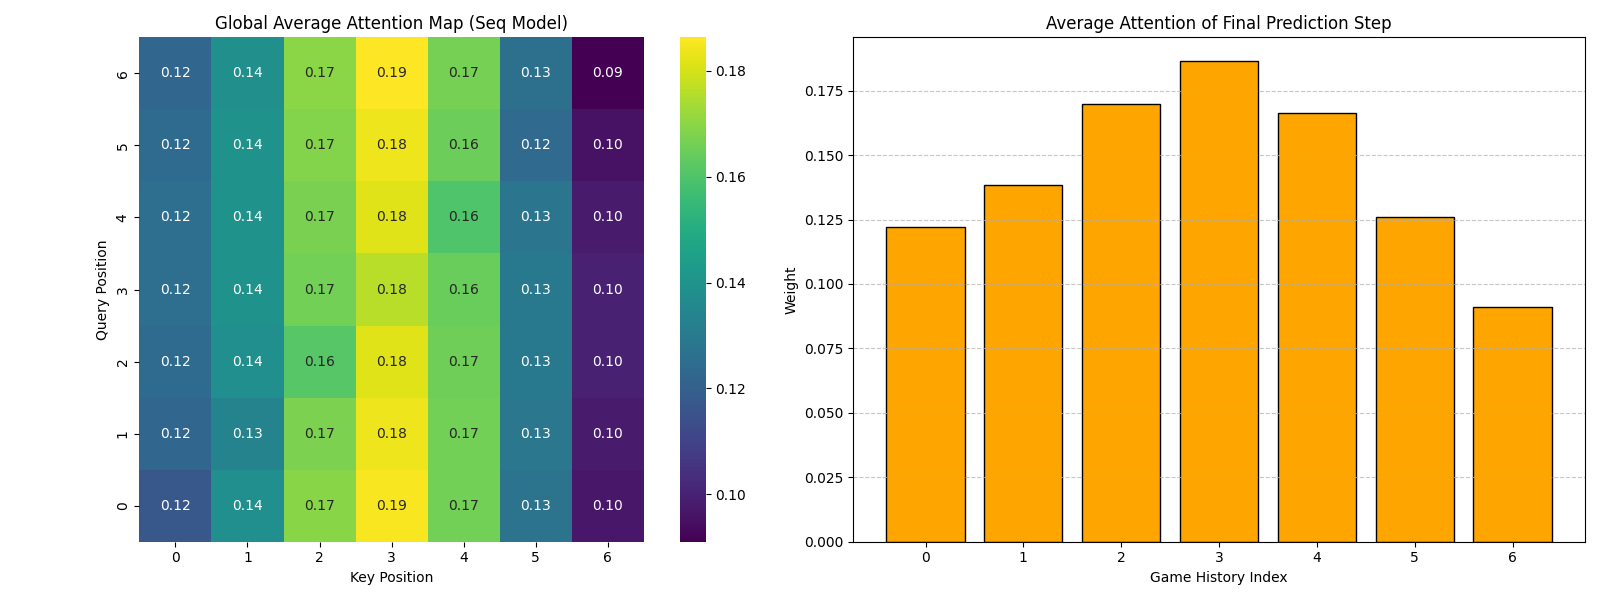
\includegraphics[width=\linewidth]{attention_aggregated.png}}
\caption{Aggregated Attention Weights of the Transformer over 7 past games.}
\label{fig:attn}
\end{figure}
Analysis of the Transformer's attention maps revealed a ''Bell-Shaped'' temporal dynamic. Weights were often highest in the middle of the sequence (games 3-5) rather than the most recent games. This suggests the model relies on a ''stabilized average form'' to anchor its predictions against extreme outliers or recent noise.

\section{Conclusion and Future Directions}
This project demonstrated that Deep Learning, specifically a Transformer-based approach, can effectively mine complex patterns from raw NBA data, achieving high performance without extensive manual feature engineering. While the integration of spatial shot heatmaps did not yield the expected improvements due to information redundancy, the implementation of Quantile Regression proved to be a critical component for practical application, transforming the prediction model into a robust risk-management tool.

Future work will focus on integrating Play-by-Play text streams and news sentiment analysis using Large Language Models (LLMs). The goal is to capture contextual nuances---such as player injury, defensive intensity, or momentum shifts---confounded in box scores, potentially advancing the prediction window from pre-game to In-Game (Live Betting).


\begin{thebibliography}{00}
\bibitem{b1} A. Vaswani et al., ''Attention is all you need,'' in Advances in neural information processing systems, 2017, pp. 5998--6008.
\bibitem{b2} NBA API, ''nba\_api,'' https://github.com/swar/nba\_api.
\bibitem{b3} Source Code, https://github.com/Nelson0314/NBA-predictor.
\end{thebibliography}

\end{document}
